\section{Распознавание и скелетизация людей}
\begin{frame}
    \frametitle{Распознавание людей и их позиций}
    \begin{figure}
        \centering
        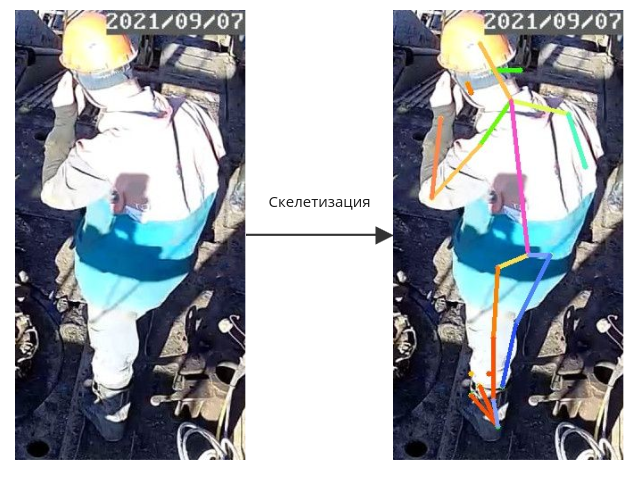
\includegraphics[width=0.9\textwidth,keepaspectratio]{skeletization}
    \end{figure}
\end{frame}

%\begin{frame}
%    \frametitle{Модель AlphaPose}
%    \begin{figure}
%        \centering
%        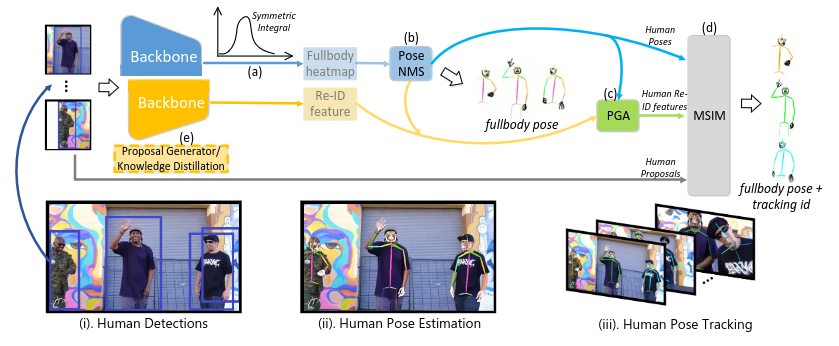
\includegraphics[width=1.0\textwidth,keepaspectratio]{alphapose_1}
%    \end{figure}
%\end{frame}

\begin{frame}
    \frametitle{Модель AlphaPose}
    \begin{figure}
        \centering
        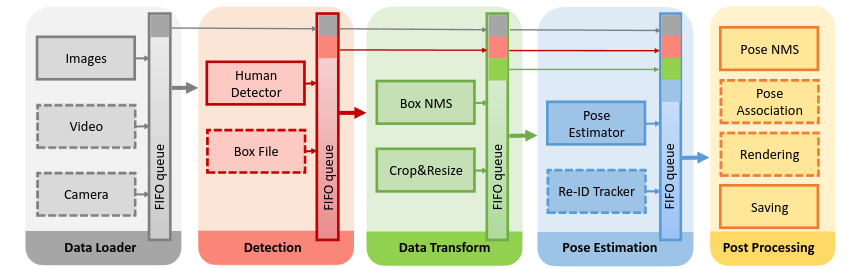
\includegraphics[width=1.0\textwidth,keepaspectratio]{alphapose_2}
    \end{figure}
\end{frame}

\begin{frame}
    \frametitle{Выходной формат данных скелетной модели}
    По заданному кадру алгоритм строит множество $\mathbf{S}$ скелетных моделей.

    Каждый элемент $\mathbf{S}$ имеет вид:
    $$ \left(ID, K, BB\right), $$
    где:
    \begin{itemize}
        \item $ID$ -- уникальный идентификатор человека в кадре
        \item $K$ -- список ключевых точек скелетной модели
        \item $BB$ -- ограничивающая рамка для изображения человека
    \end{itemize}
\end{frame}

\begin{frame}
    \frametitle{Формат представления ключевых точек}
    $$ K = [(x_i, y_i, c_i)]_{i=0}^{N-1}, $$
    где
    \begin{itemize}
        \item $(x_i, y_i)$ -- координаты ключевой точки на изображении
        \item $c_i$ -- уверенность алгоритма, что ключевая точка предсказана корректно
        \item $N$ -- общее число ключевых точек (26~тело, 21~левая~рука, 21~правая~рука)
    \end{itemize}
\end{frame}

\begin{frame}
    \frametitle{Нумерация ключевых точек}
    \begin{figure}
        \begin{minipage}[!h]{0.49\linewidth}
            \centering
            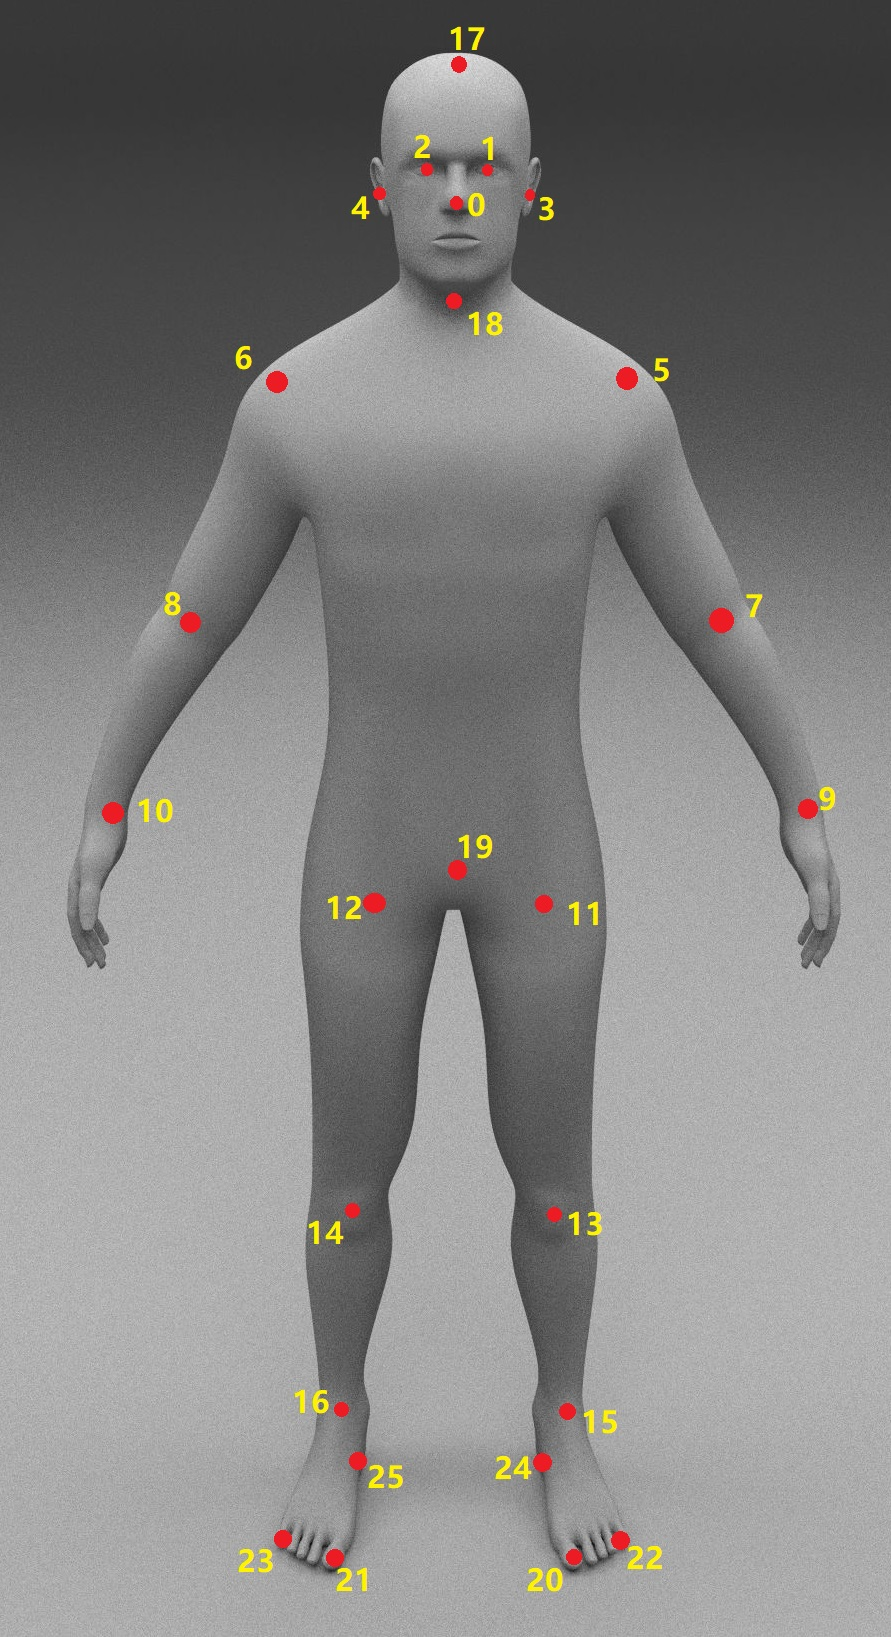
\includegraphics[width=0.7\textwidth,keepaspectratio]{keypoints_map_1}
        \end{minipage}
        \hfill
        \begin{minipage}[!h]{0.49\linewidth}
            \centering
            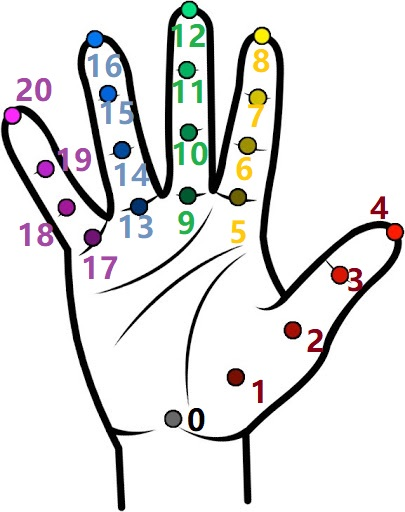
\includegraphics[width=0.7\textwidth,keepaspectratio]{keypoints_map_2}
        \end{minipage}
    \end{figure}
\end{frame}